\capitulo{5}{Aspectos relevantes del desarrollo del proyecto}

Este apartado pretende recoger los aspectos más importantes del desarrollo del proyecto. Se tratará de exponer el camino que se ha tomado con sus correspondientes implicaciones, así como describir los diferentes problemas a
los que ha habido que enfrentarse y las soluciones con las que se ha tratado de resolverlos.

\section{Inicio del proyecto}

Me considero una persona con muchas inquietudes y siempre pensando en mejorar tareas que suelo realizar con mucha frecuencia. He desarrollado mi carrera profesional en el campo de la Topografía y la Geodesia, y actualmente está mas enfocado a temas relacionados con la Cartografía.

Trabajando en varios proyectos, he podido observar la cantidad de tiempo y recursos que se empleaban, en realizar levantamientos topográficos y posteriormente gestionar todos esos datos para producir un plano. De ahí surge la idea de como mejorar el trabajo de campo mediante un tipo de codificación,  y que esta a su vez sirviera para automatizar al máximo el proceso de delineación, a la hora de  crear el plano.

El profundizar en los conocimientos adquiridos cursando el Grado en Ingeniería Informática y a la vez poder facilitar el trabajo en este tipo de proyectos, me ha animado a hacer viable este proyecto. A la hora de decidirme, también me ha parecido importante, la idea de que la aplicación desarrollada es de gran utilidad, y seguro que va a ser bien recibida por la comunidad de topógrafos.

La idea fue aceptada por los tutores, y comenzamos con el proyecto.

\begin{figure}[!h]
	\centering
	
\includegraphics[width=0.4\textwidth]{SPC}
	\caption{Logo de \emph{SurveyingPointCode}.}
	\label{fig:SPC}
\end{figure}


\section{Gestión del proyecto}

En la primera reunión con los tutores, se estableció cual iba a ser la metodología a seguir en la realización de este proyecto. Se iba a emplear la metodología ágil \emph{Scrum}.

Se realizarían una serie de \emph{sprints} llevados a cabo con una periodicidad media semanal, donde se entregaría una parte del producto operativo, el incremento. Al finalizar cada \emph{sprint} se realizarían reuniones para planificar las tareas a realizar en el el \emph{sprint} siguiente, en forma de pila del \emph{sprint}, y revisar si se habían alcanzado los objetivos marcados en el \emph{sprint} anterior.

En \emph{GitHub}, con la herramienta \emph{ZenHub}, se visualizarían el estado y prioridad de las tareas del \emph{sprint}. Los avances y cambios en el desarrollo del proyecto, se almacenaría en \emph{GitHub}, que nos permitiría seguir al detalle  todo el histórico del proyecto.

Las reuniones de los \emph{sprints} resultaron muy interesantes. En ellas hubo modificaciones sobre la idea inicial de la que se partía, en algunos casos desechado alguna funcionalidad, como la de incorporar un visor para poder visualizar el plano en el navegador (véase la explicación en el \emph{sprint} 6, en el anexo), pero en la mayoría de los casos, aportando nuevas funcionalidades que hacían  crecer el valor de la aplicación, y sobre todo me aportaron una visión más realista a la hora de abordar unos determinados objetivos o ideas, preguntándome, si el tiempo o recursos invertidos merecían la pena o aportaban algún valor a la aplicación.

\section{Formación}

La realización del proyecto requería una serie de conocimientos técnicos, en general, en el desarrollo de aplicaciones web,y en particular en  tecnologías como;
Flask, HTML5, CSS3, JavasScript, Docker y bilbliotecas como \texttt{Ply}, \texttt{ezdxf}, \texttt{Boostrap}, \texttt{TinyColor},...

Los mayores esfuerzos se pusieron en comprender el funcionamiento de Flask, \texttt{Ply}, \texttt{ezdxf} y Docker, ya que el óptimo funcionamiento de la aplicación  en estos puntos, era fundamental para logar conseguir los objetivos finales. 

Como la aplicación se ha desarrollado en Python, era importante conocer las guías de estilo y la convenciones de este lenguaje, \textbf{PEP 8} y \textbf{PEP 257} entre otras. Para ello se consultaron las siguientes fuentes:

\begin{itemize}
\item PEP 8 -- Style Guide for Python Code \cite{PEP8}
\item PEP 257 -- Docstring Conventions \cite{PEP257}
\end{itemize}


Para la formación en \textbf{Flask} se consultaron las siguientes fuentes:

\begin{itemize}
\item Building Web Applications  with Flask \cite{Flask1}
\item Instant Flask Web Development \cite{Flask2}
\end{itemize}

Para la formación en \textbf{Ply} se consultaron las siguientes fuentes:

\begin{itemize}
\item Documentation for PLY  \cite{HomePly}
\item Prototyping Interpreters using Python Lex-Yacc \cite{Ply2}
\item Parses chemical equations using the PLY parser generator \cite{Ply3}
\end{itemize}

Para la formación en \textbf{ezdxf} y las otras posibles alternativas,se consultaron las siguientes fuentes:

\begin{itemize}
\item Documentation for ezdxf \cite{ezdxf}
\item Documentation for dxfgrabber \cite{dxfgrabber}
\item Documentation for dxfwrite \cite{dxfwrite}
\item Documentation for SDXF \cite{sdxf}
\end{itemize}

Para la formación en \textbf{SQLAlquemy}  y \textbf{Flask-Login}, se consultaron las siguientes fuentes:

\begin{itemize}
\item Documentation for SQLAlquemy \cite{SQLAlquemy}
\item Documentation for Flask-Login \cite{Flasklogin}
\end{itemize}

Para la formación en \textbf{HTML5} se consultaron las siguientes fuentes:

\begin{itemize}
\item HTML5 Tutorial \cite{html5}
\end{itemize}

Para la formación en \textbf{CSS3} se consultaron las siguientes fuentes:

\begin{itemize}
\item CSS Tutorial \cite{css3}
\item Lenguaje CSS \cite{css3_1}
\end{itemize}

Para la formación en \textbf{JavaScript} se consultaron las siguientes fuentes:

\begin{itemize}
\item Eloquent JavaScript: A Modern Introduction to Programming \cite{JavaScript}
\item Javascript a fondo \cite{JavaScript_1}
\end{itemize}

Para la formación en \textbf{Bootstrap} y bilbliotecas relacionadas, se consultaron las siguientes fuentes:

\begin{itemize}
\item Bootstrap \cite{Bootstrap}
\item TinyColor JavaScript color tooling \cite{TinyColor}
\item Bootstrap Colorpicker \cite{Colorpicker}
\item jquery.cookie \cite{j-cookie}
\end{itemize}


Para la formación en \textbf{Docker} se consultaron las siguientes fuentes:

\begin{itemize}
\item Curso Docker \cite{Docker}
\item Docker for beginners \cite{Docker_1}
\item Introduction to Docker \cite{Docker_2}
\item Docker-postgis \cite{Docker_3}
\item Overview of Docker Compose \cite{Docker_4}
\end{itemize}

\section{Desarrollo de la aplicación}

Los primeros pasos en el desarrollo de la aplicación consistieron en desarrollar un pequeño prototipo funcional, que fuera incrementando su funcionalidad progresivamente.

El primer prototipo, tenía que conseguir leer un archivo de campo y darlo por válido o como erróneo. Una vez que se tuvo clara como iba a ser la codificación de cada punto, (según hemos visto en la Sección~\ref{sec:codificacion} en la página~\pageref{sec:codificacion}), el siguiente paso era definir una gramática para ese tipo de archivo, para poder validarla. Entre los formatos de archivo más comunes que podemos obtener de los equipos topográficos, se decidió que los archivos deberían ser de tipo <<csv>> o <<txt>>, separando sus campos por comas. Los campos son; número de punto, coordenada $x$, coordenada $y$, coordenada $z$ y código del punto. 

A continuación, vemos un ejemplo, con todas las posibilidades de codificación que aceptará la aplicación: 
\begin{verbatim}


1,355776.180,4611015.011,691.055,E I
2,355773.203,4611028.546,691.055,E
3,355781.359,4611129.076,691.055,TR REG
4,355786.052,4611135.542,691.055,TC TEL
5,355783.215,4611143.179,691.055,TX 2 SAN
6,355754.037,4611145.893,691.055,A IC
7,355755.345,4611150.953,691.055,A C
8,355857.822,4611095.993,691.055,E -14.1 20.5 -25.75
\end{verbatim}



Se estudió detenidamente esta sintaxis y la formalización de la gramática quedó de la siguiente forma:

\begin{verbatim}
entrada: líneas

líneas: línea | líneas '\n' línea

línea: núm_punto coordenadas código

núm_punto: INT

coordenadas: FLOAT, FLOAT, FLOAT

INT: [0-9]+

FLOAT: -?( [0-9]*.[0-9]+)

ID: [a-zA-Z]+

código: código_capa CÓDIGO_GEOMÉTRICO
      | CÓDIGO_ELEMENTO_SINGULAR código_valor_texto
      | código_capa código_no_accesible
      | código_elemento_singular
      | código_capa      
      
código_capa: ID

CÓDIGO_GEOMÉTRICO: "I" | "IC" | "C"

CÓDIGO_ELEMENTO_SINGULAR: "TC" | "TR" | "TX"

código_valor_texto: FLOAT ID
                  | INT ID
                  | FLOAT
                  | INT
                  | ID       
                                 
código_no_accesible: (FLOAT | INT)+
\end{verbatim}

El prototipo utilizando la biblioteca \texttt{Ply} y con esta gramática,  consiguió validar un archivo correcto.

Otro punto clave en el desarrollo del algoritmo fue descifrar los códigos que contenía el archivo de entrada. Como se ha comentado anteriormente, este código puede tener distintos significados dependiendo de su estructura, por ejemplo:

\begin{itemize}
\item AR, puede ser un punto que se guarde en una futura capa llamada Árboles.
\item TX 2 SAN, puede ser un punto que es el centro de un circulo de radio 2 y que se guarde en una futura capa llamada Saneamiento.
\item M I, puede ser un punto donde comienza una línea que define un muro y que se guarde en una futura capa llamada Muros.
\item …
\end{itemize}

El algoritmo debía extraer del archivo todos los elementos, identificarlos y guardarlos en alguna estructura de datos, clasificados por:

\begin{itemize}
\item Capas
\item Puntos
\item Líneas
\item Curvas
\item Cuadrados
\item Rectángulos 
\item Círculos
\end{itemize}

Añadiendo complejidad al archivo de entrada, se comprobó que el algoritmo resolvía de forma satisfactoria este paso.

Por último, para poder tener un prototipo básico que cumpliera los objetivos, debíamos comprobar que el prototipo era capaz de crear un archivo \textbf{DXF}, con los elementos del archivo de entrada. Incorporando la biblioteca \texttt{ezdxf}, y haciendo uso de sus métodos y atributos, se testó que dibujara en un primer momento solo líneas y curvas, siendo capaz de generarlas en el orden correcto.

Con estos datos de entrada:

\begin{verbatim}

1,355776.180,4611015.011,691.055,E I
2,355773.203,4611028.546,691.055,E
3,355761.305,4611083.365,691.055,E
4,355767.050,4611086.462,691.055,A I
5,355774.447,4611083.001,691.055,M I
6,355769.692,4611104.977,691.055,M
7,355763.294,4611103.572,691.055,A
8,355756.420,4611105.247,691.055,E
9,355781.359,4611129.076,691.055,TR RE
10,355782.355,4611131.314,691.055,TR RE
11,355788.919,4611128.392,691.055,TR RE
12,355766.146,4611121.294,691.055,M
13,355759.713,4611119.882,691.055,A
14,355750.443,4611133.259,691.055,E
15,355786.052,4611135.542,691.055,TC TEL
16,355786.849,4611136.145,691.055,TC TEL
17,355764.814,4611134.156,691.055,ARB
18,355783.215,4611143.179,691.055,TX 0.5 SAN
19,355761.943,4611140.629,691.055,M
20,355755.486,4611139.240,691.055,A
21,355754.037,4611145.893,691.055,A IC
22,355745.977,4611153.511,691.055,E
23,355755.345,4611150.953,691.055,A C
24,355758.897,4611153.511,691.055,A C
\end{verbatim}

El resultado fue:

\imagen{proto_1}{Dibujo obtenido con el prototipo inicial}


Es resultado fue el esperado, por lo que se concluyó esta primera etapa del desarrollo con un pequeño prototipo que cumplía las funcionalidades previstas inicialmente:

\begin{itemize}
\item Leer y validar un archivo con una gramática determinada.
\item Interpretar y organizar todos los elementos del archivo, a partir de su codificación.
\item Crear un archivo DXF con estos elementos.
\end{itemize}

A partir de aquí, como ya se había decidido que iba a ser una aplicación Web, el próximo objetivo era desarrollar la aplicación Web con \textbf{Flask}. El proceso iba a ser el mismo que con el prototipo anterior, desarrollar un prototipo de aplicación Web que fuera incrementando sus funcionalidades.

A continuación, se enumeran brevemente y ordenadas temporalmente, las funcionalidades más importantes que se han ido añadiendo al prototipo Web:
\begin{itemize}
\item Subir un archivo al servidor.
\item Procesar y descargar un archivo al equipo del usuario.
\item Conexión con una BBDD. (en este punto se comenzó a trabajar con Docker, la BBDD iba dentro de un contenedor).
\item \emph{Login}, \emph{Logout} y Registro. Para implementar esta parte se trabajó con la biblioteca \texttt{Flask-Login}.
\item Sesiones de usuarios. 
\end{itemize}

Estas funcionalidades cubrían las expectativas de que la aplicación fuera una aplicación Web, el prototipo Web ya se había conseguido.

A partir de aquí, se han ido desarrollando todas las funcionalidades de la aplicación tanto en \emph{Frontend} como en  \emph{Backend}.

\section{Problemas, incidencias y soluciones}

A continuación, se exponen algunos  problemas surgidos, incidencias y como se abordaron.


\subsubsection{Conflicto entre \emph{parsers}}

Tras obtener el prototipo inicial, con la funcionalidad que se tenía en mente en un principio,  surgió la idea que el usuario pudiera subir un archivo con una configuración personalizada para hacer la conversión de archivo de campo a archivo DXF. 

Como podemos ver en la Tabla~\ref{tabla:config}, relacionamos códigos de punto, con capas de CAD, colores y símbolos. Cuando exista un trabajo con múltiples códigos, capas y colores, se quiere dar al usuario la posibilidad de no tener que configurar cada vez esta conversión en la interfaz, sino que a través de un archivo personalizado, con sus códigos, capas, colores y símbolos, esta parte sea también automática.

\tablaSmall{Esquema archivo de configuración}{l c c c
}{config}
{ \multicolumn{1}{l}{Código de punto} & Capa de CAD & Color & Símbolo \\}{ 
E & Edificación & Rojo\\
AR & Vegetación & Verde & Árbol\\
SAN & Saneamiento & Amarillo \\
P & Saneamiento & Amarillo & Pozo \\
}

Para ello se formalizó otra gramática para validar este tipo de archivos y detectar sus errores. La gramática elegida fue la siguiente:


\begin{verbatim}

entrada: líneas

líneas: línea | líneas '\n' línea

línea: TEXT COMA TEXT COMA color COMA TEXT
     | TEXT COMA TEXT COMA color
     
color: LPAREN INT COMA INT COMA INT RPAREN

TEXT: [a-zA-Z0-9_]+

INT: [0-9]+

LPAREN = '\('

RPAREN = '\)'

\end{verbatim}

Los \emph{parsers} estaban definidos en diferentes módulos, el \emph{parser} para el archivo del campo estaba en módulo \ruta{conversor.py} y el del archivo de configuración en el módulo \ruta{upload\_optional\_files.py}. Cuando se ejecutan, se crean los archivos \ruta{parser.out} y \ruta{parsetab.py}. Probando a cargar los dos archivos a la vez, se pudo comprobar que se parseaba un archivo con el \emph{parser} que no le correspondía. Esto no sucedía siempre, si no que pasaba  de una forma aleatoria, como si en algún momento se cruzara la información entre \emph{parsers}.

Se solucionó esta parte añadiendo un parámetro personalizado para cada tipo de \emph{parser}. En un principio estaba definido de esta forma para ambos casos:
\

\begin{lstlisting}
lex.lex() # lexer part
...
punto = parser.parse(line) # parser part
\end{lstlisting}

Definiendo parámetros independientes en cada caso, quedó de la siguiente forma.

Para el archivo de campo:

\begin{lstlisting}
lexer_topographycal=lex.lex() # lexer part
...
# añadiendo el nuevo parámetro
punto = parser.parse(line,lexer=lexer_topographycal)
\end{lstlisting}
\newpage
Para el archivo de configuración:

\begin{lstlisting}
lexer_config = lex.lex() # lexer part
...
# añadiendo el nuevo parámetro
c_line = parser.parse(line, lexer=lexer_config)
\end{lstlisting}
Para dar con esta solución, se consultó la documentación de \texttt{Ply}, concretamente el apartado \textbf{Multiple Parsers and Lexers} \cite{Parser}.


\subsubsection{Codificación \texttt{UTF-8}}

Hasta ahora la aplicación funcionaba correctamente a la hora de subir los archivos y validarlos. Se decidió modificar la gramática del archivo de configuración, para que aceptará la letra <<ñ>> y todos los tipos de tildes, ya que se suelen utilizar al poner los nombres de las capas de CAD. 

Simplemente se sustituyó:

\begin{verbatim}
TEXT: [a-zA-Z0-9_]+
\end{verbatim}

por: 

\begin{verbatim}
TEXT: [a-zA-ZÀ-ÿ0-9ñÑ_]+
\end{verbatim}


Con esto debería funcionar perfectamente, pero no fue así, el archivo que contenía el carácter <<ñ>>, daba errores. Se estaba probando la aplicación simultáneamente en 2 sistemas operativos Windows y Linux, y para mayor sorpresa en Linux funcionaba y en Windows no.

Al final, se dedujo que se podía tratar de un problema de codificación del archivo, e investigando en esa línea decidimos probar dos configuraciones, \texttt{UTF-8} y \texttt{Latin-1}, en los 2 sistemas , y en cada uno sucedía lo contrario, como se puede ver en la Tabla Tabla~\ref{tabla:WL}


\tablaSmall{Test Windows vs Linux para \texttt{UTF-8} y \texttt{Latin-1}}{l c c c
}{WL}
{ \multicolumn{1}{l}{Sistema Operativo} & UTF-8 & Latin-1 \\}{ 
Windows & Fallo & Correcto\\
Linux & Correcto & Fallo\\
}
 
La solución encontrada fue añadir en la función que abre el archivo, el parámetro \emph{encoding} indicando el tipo de codificación específicamente , en este caso \texttt{UTF-8}. 

En el código se sustituyó:
\begin{lstlisting}
  with open(input_file) as f:
\end{lstlisting}

por:
\begin{lstlisting}
  with open(input_file, encoding='utf-8') as f:
\end{lstlisting}

Se comprobó en ambos sistemas operativos, y el resultado fue correcto, así que se dio esta solución como válida.


\subsubsection{Paleta de colores en CAD}

Una funcionalidad importante de la aplicación es poder asignar un color a una capa de CAD, así todos los elementos pertenecientes a esa capa se dibujarán en ese color. 

La función para crear una nueva capa de la biblioteca \texttt{ezdxf},

\begin{lstlisting}
  dwg.layers.new(nombre_capa, dxfattribs={'color': 1})
  # atributo color, en este ejemplo igual a 1
\end{lstlisting}

\noindent solo permite colores entre 0 y 255, por lo que en un principio, se pensó en usar esta paleta de colores o si la entrada se producía en formato RGB, tanto en el archivo de configuración o a través de la interfaz, se transformaría de RGB a 256 colores, mediante la siguiente trasformación:

\begin{lstlisting}
def rgb(r,g,b):
    grayP=True
    gray=False
    sep=45.5

    while(grayP):
        if (r<sep)or g<sep or b<sep:
            gray=r<sep and g<sep and b<sep
            grayP=False
        sep+=42.5

    if (gray):
        return round(232+(r+g+b)/33)
    else:
        return 16+(6*r/256)*36+(6*g/256)*6+(6*b/256
\end{lstlisting}

El algoritmo anterior se consultó en:

\url{https://github.com/janlelis/paint} 

Con esto se había solucionado el problema, ya teníamos cada capa con su correspondiente color.

Al cabo de bastantes pruebas, apareció un detalle que en un principio me había pasado inadvertido, los colores que seleccionaba el usuario para crear el archivo DXF en la aplicación , no se correspondían con los que realmente se visualizaban en el dibujo, una vez abierto con un programa de CAD.

Investigando, se averiguó que los programas de CAD tienen su propia paleta de colores, que fue creada por AutoCAD, donde a cada color se le asigna un número entero entre 0 y 255. En el siguiente enlace se puede consultar:


\url{http://gohtx.com/acadcolors.php}

Esta parte se solucionó incluyendo en la aplicación, una lista con estos colores, donde se comparaba el RGB definido por el usuario con el de la lista, y si existía, devolvía el número entero correspondiente a la paleta de CAD.

Cuando los colores estaban definidos en el archivo de configuración, no había problema, era una conversión directa usando la lista anterior, pero si el usuario deseaba asignar o modificar el color a través de la interfaz, el color que él había seleccionado debería ser igual al que apareciera en el dibujo. Para ello se utilizó la biblioteca de JavaScript, \texttt{TinyColor}, que nos permite personalizar la paleta de colores con cualquier lista que le proporcionemos.

\imagen{colores_cad}{Ejemplo diez primeros colores en la paleta de colores CAD}

\imagen{colores_app}{Paleta de colores de \emph{SurveyingPointCode}}

En las figuras~\ref{fig:colores_cad} y ~\ref{fig:colores_app}, se puede observar que la disposición de colores está ordenada de la misma forma, coincidiendo su posición con el número entero correspondiente al color de la paleta de CAD.

\subsubsection{Versiones iniciales de CAD}

En un principio de planteó que la aplicación debería poder generar versiones de archivos DXF compatibles con todas las versiones de CAD existentes en el mercado.

En los prototipos iniciales, con los ejemplos de archivos de campo que veníamos trabajando, se comprobó que se generaban archivos DXF válidos para todas las versiones de CAD. Hasta ahora se habían utilizado elementos de CAD, de tipo:

\begin{itemize}
\item \texttt{POINT}
\item \texttt{LWPOLYLINE}
\item \texttt{CIRCLE}
\item \texttt{SPLINE}
\item \texttt{TEXT}
\end{itemize}

Que permitían esta compatibilidad, con las versiones más antiguas.   

La aplicación en un principio estaba pensada para que el usuario pudiera asociar   a determinados códigos de puntos, un símbolo. Por ejemplo, en un punto que tuviera el código AR, debía dibujar un árbol.(Véase un ejemplo de distintos símbolos en la Figura~\ref{fig:Simbolos}).

Se añadió esta nueva funcionalidad, que debía realizar los siguientes pasos:

\begin{itemize}
\item Subir un archivo DXF con bloques.
\item Extraer los bloques que contiene ese archivo.
\item Incorporar esos bloques a nuestro dibujo.
\item Asignar esos bloques a determinados puntos, para que sean dibujados como símbolos.
\end{itemize}

Y el nuevo tipo de elemento añadido \texttt{BLOCK}, hizo que versiones mas antiguas de CAD, no soportaran este formato.

Valorando este problema, se determinó que era mejor desechar el poder trabajar con versiones más antiguas de CAD, en favor, de que el usuario pudiera asignar símbolos al dibujo. Sin esta posibilidad, la aplicación perdería mucho valor.


\begin{figure}[!h]
	\centering
	\includegraphics[width=0.6\textwidth]{cad_versions_ok}
	\caption{Versiones de CAD aceptadas por \emph{SurveyingPointCode}.}
	\label{fig:cad_versions_ok}
\end{figure}


En la Figura~\ref{fig:cad_versions_ok}, podemos ver las versiones de archivos DXF
compatibles en \emph{SurveyingPointCode}

\subsubsection{Despliegue de la aplicación --- Docker Compose.}

Como idea inicial, se planteó el uso de Docker para llevar a cabo el despliegue de la aplicación. Una vez que tengamos bien configurados los contenedores, es sencillo de desplegar en cualquier equipo.

Primero, se configuró el contenedor  de la base de datos, \emph{PostGIS}, junto con \emph{PgAdmin4}, para gestionar la base de datos. Dos contenedores conectados entre sí.

Mas adelante, se pensó crear un contenedor que contuviera la aplicación, configurar un contenedor con \emph{Flask}. Ya teníamos tres contenedores independientes conectados entre sí, y con la aplicación funcionando perfectamente.

Para desplegar la aplicación, había que descargar la imagen de cada contenedor, crear y arrancar cada contenedor, individualmente. Consultando información, comprobamos que existía una forma mejor de hacerlo, utilizando \textbf{Docker Compose}. 

\textbf{Docker Compose} es una herramienta que permite simplificar el uso de \emph{Docker} generando \emph{scripts} que facilitan el diseño y la construcción de servicios. Se pueden crear diferentes contenedores y al mismo tiempo, en cada contenedor, diferentes servicios.

En el archivo \texttt{docker-compose.yml}, se configuran los contenedores y las relaciones que existen entre ellos. A continuación podemos ver el archivo \texttt{docker-compose.yml} utilizado.

\begin{lstlisting}
version: '2.1'
services:
  postgis:
    image: 'mdillon/postgis'
    container_name: postgis
    environment:
      - POSTGRES_USER=${POSTGRES_USER}
      - POSTGRES_PASS=${POSTGRES_PASS}
      - POSTGRES_DBNAME=${POSTGRES_DBNAME}
      - ALLOW_IP_RANGE=${ALLOW_IP_RANGE}
    networks:
      - pgnetwork
    volumes:
      - 'pg_data:/var/lib/postgresql'
    ports:
      - '5432:5432'
    hostname: postgis  
    restart: always
  pgadmin:
    image: 'dpage/pgadmin4'
    ports:
      - '80:80'
    volumes:
      - 'pga4volume:/var/lib/pgadmin'
    container_name: pgadmin4
    networks:
      - pgnetwork
    environment:
      - PGADMIN_DEFAULT_EMAIL=${PGADMIN_DEFAULT_EMAIL}
      - PGADMIN_DEFAULT_PASSWORD=
      	${PGADMIN_DEFAULT_PASSWORD}
    depends_on:
      - postgis
  flask:
    build: . 
    ports:
      - "5000:5000"
    volumes:
      - .:/SurveyingPointCode
    links:
      - postgis:postgres 
    container_name: surveying_point_code
    environment:
      - POSTGRES_USER=${POSTGRES_USER}
      - POSTGRES_PASS=${POSTGRES_PASS}
      - POSTGRES_DBNAME=${POSTGRES_DBNAME}   
      - POSTGRES_HOST=${POSTGRES_HOST}
      - POSTGRES_PORT=${POSTGRES_PORT} 
    networks:
      - pgnetwork
    restart: always  
\end{lstlisting}

\noindent\texttt{postgis}, \texttt{pgadmin} y \texttt{flask}, son los tres servicios que vamos a utilizar. Con el parámetro \texttt{container\_name}, definimos el nombre de los contenedores y con el parámetro \texttt{image}, la imagen que queremos usar para crear ese contenedor. Los parámetros \texttt{depends\_on} y \texttt{links}, indican las relaciones y dependencias entre los contenedores. Otros parámetros importantes son: \texttt{ports},\texttt{ networks},\texttt{ environment},\texttt{ volumes}, etc.


En la tabla siguiente se pueden ver los servicios que se ofrecen en el archivo \texttt{docker-compose.yml}.

\begin{longtable}[]{@{}llll@{}}
\toprule
\begin{minipage}[b]{0.18\columnwidth}\raggedright\strut
Servicio\strut
\end{minipage} & \begin{minipage}[b]{0.30\columnwidth}\raggedright\strut
Imagen\strut
\end{minipage} & \begin{minipage}[b]{0.30\columnwidth}\raggedright\strut
Contenedor\strut
\end{minipage} & \begin{minipage}[b]{0.11\columnwidth}\raggedright\strut
Puerto\strut
\end{minipage}\tabularnewline
\midrule
\endhead
\begin{minipage}[t]{0.18\columnwidth}\raggedright\strut
\texttt{postgis}\strut
\end{minipage} & \begin{minipage}[t]{0.30\columnwidth}\raggedright\strut
\texttt{mdillon/postgis}\strut
\end{minipage} & \begin{minipage}[t]{0.30\columnwidth}\raggedright\strut
\texttt{postgis}\strut
\end{minipage} & \begin{minipage}[t]{0.11\columnwidth}\raggedright\strut
5432\strut
\end{minipage}\tabularnewline
\begin{minipage}[t]{0.18\columnwidth}\raggedright\strut
\texttt{pgadmin}\strut
\end{minipage} & \begin{minipage}[t]{0.30\columnwidth}\raggedright\strut
\texttt{dpage/pgadmin4}\strut
\end{minipage} & \begin{minipage}[t]{0.30\columnwidth}\raggedright\strut
\texttt{pgadmin4}\strut
\end{minipage} & \begin{minipage}[t]{0.11\columnwidth}\raggedright\strut
80\strut
\end{minipage}\tabularnewline
\begin{minipage}[t]{0.18\columnwidth}\raggedright\strut
\texttt{flask} \strut
\end{minipage} & \begin{minipage}[t]{0.30\columnwidth}\raggedright\strut
\texttt{python:3.7-alpine}\strut
\end{minipage} & \begin{minipage}[t]{0.30\columnwidth}\raggedright\strut
\texttt{surveying\_point\_code}\strut
\end{minipage} & \begin{minipage}[t]{0.11\columnwidth}\raggedright\strut
5000\strut
\end{minipage}\tabularnewline
\bottomrule
\caption{Servicios incluidos en \texttt{docker-compose.yml}}
\end{longtable}

El servicio de \texttt{flask} es algo mas complejo, ya que no es solo utilizar un contenedor que permita Python, si no que debemos alojar nuestra aplicación en él. Para ello hemos utilizado el archivo \texttt{Dockerfile}, donde definimos , la version de Python a utilizar, así como la estructura que tendrá dentro del contenedor la aplicación y los requerimientos necesarios para su funcionamiento.
A continuación, vemos este archivo:
\newpage
\begin{lstlisting}
FROM python:3.7-alpine

RUN mkdir /SurveyingPointCode

WORKDIR /SurveyingPointCode

ADD . .

RUN apk update && apk add postgresql /
		-dev gcc python3-dev musl-dev
RUN pip install -r requirements.txt
	
EXPOSE 5000

ENV FLASK_APP=surveyingpointcode.py

CMD ["flask", "run", "--host=0.0.0.0"] 
\end{lstlisting}

Si nos fijamos en el archivo \texttt{docker-compose.yml}, el servicio \texttt{flask} no tiene el parámetro \texttt{image}, en su defecto tiene el parámetro  \texttt{build} y el valor del parámetro es un punto, <<\texttt{build: .}>>. Con esto le estamos indicado que construya ese contenedor, con el archivo \texttt{Dockerfile} que encuentre en ese directorio.

Por último, y gracias a la utilización de \textbf{Docker Compose} toda la aplicación se despliega con con solo comando, \texttt{docker-compose up}, este comando descarga las imágenes, construye los contenedores y los arranca.

Para facilitar el despliegue, en este proyecto se han implementado dos \texttt{scripts}.

El primero, \textbf{\texttt{app\_install.sh}}, lo vemos a continuación:
\begin{lstlisting}
#!/bin/bash
. ./app-env

docker-compose up -d postgis
until docker exec -it postgis psql 
  --username=${POSTGRES_USER}
  --dbname=${POSTGRES_DBNAME} -c '\q'; do
	echo "Postgis is uniavaliable...sleeping"
	sleep 1
done
echo "Postgis is up"
docker-compose up -d flask
\end{lstlisting}

Este \texttt{script} arranca la aplicación con los contenedores \texttt{surveying\_point\_code} y \texttt{postgis}.

El segundo \texttt{script}, \textbf{\texttt{app\_install\_pgadmin.sh}}:

\begin{lstlisting}
#!/bin/bash
. ./app-env

docker-compose up -d postgis
until docker exec -it postgis psql
  --username=$POSTGRES_USER} 
  --dbname=${POSTGRES_DBNAME} -c '\q'; do
	  echo "Postgis is uniavaliable...sleeping "
      sleep 1
done
echo "Postgis is up"
docker-compose up -d flask pgadmin
\end{lstlisting}

Este otro \texttt{script} arranca aplicación con los contenedores \texttt{surveying\_point\_code}, \texttt{postgis} y \texttt{pgadmin}.

La razón de implementar estos \texttt{scripts}, es que se ha comprobado que al ejecutar la aplicación en diferentes equipos, en algunos casos, el contenedor \textbf{surveying\_point\_code} intentaba la conexión con la base de datos alojada en el contenedor \textbf{postgis}, antes de que estuviera creada, por lo que si se ejecutaba solamente \texttt{docker-compose up}, había que comprobar si estaba el contenedor 
\texttt{surveying\_point\_code} arrancado y si no lo estaba, había que arrancarlo manualmente mediante este comando, \texttt{docker start surveying\_point\_code}.  El uso de cualquiera de los dos \texttt{scripts} anteriores previene este caso, pues comprueba que esté creada la base de datos y después crea el contenedor \texttt{surveying\_point\_code}, que establece está conexión y permanecerá arrancado.

Aunque anteriormente se han enumerado algunas ventajas de usar Docker, aquí vamos 
a destacar la portabilidad y el despliegue rápido.
\begin{itemize}
\item Portabilidad: Una vez configurados los contenedores los podremos desplegar en fácilmente cualquier equipo solo contener instalado Docker. Los principales proveedores de computación en nube, incluidos Amazon Web Services (AWS)\footnote{\textsl{AWS}: \url{https://aws.amazon.com/es/}} y Google Compute Platform (GCP)\footnote{\textsl{GCP}: \url{https://cloud.google.com/?hl=es}}, han adoptado la disponibilidad de utilizar Docker. Docker también funciona muy bien con otros proveedores como Microsoft Azure\footnote{\textsl{Microsoft Azure}: \url{https://azure.microsoft.com/es-es/}} y OpenStack\footnote{\textsl{OpenStack}: \url{https://www.openstack.org/}}.
\item Despliegue rápido: Docker logra reducir la implementación a segundos. Esto se debe al hecho de que crea un contenedor para cada proceso y no arranca un sistema operativo. Los datos se pueden crear y destruir sin preocuparse del coste de volver a hacerlo.
\end{itemize}

\section{Análisis de la calidad del código generado}

Una vez desarrollada la aplicación se ha procedido a analizar la calidad del código mediante la herramienta \emph{Codebeat}. El resultado obtenido se puede ver en la siguiente imagen:

\begin{figure}[!h]
	\centering
	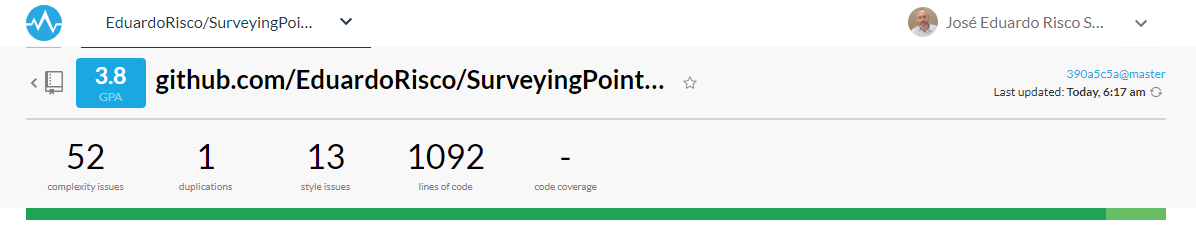
\includegraphics[width=1\textwidth]{CB_1}
	\caption{Resultado del 1º análisis con \emph{Codebeat}.}
	\label{fig:CB_1}
\end{figure}

Sobre un total de 1.092 líneas de código (estás solo son las  líneas implementadas en la aplicación, no se tienen en cuenta las librerías externas utilizadas de \emph{JavaScript} o \emph{CSS}, que se han excluido del análisis en el archivo \texttt{.codebeatignore)}, se ha obtenido una puntuación de 3,8 sobre 4. Es una puntuación bastante buena que indica un correcto desarrollo del código.

\emph{Codebeat} nos informa de la existencia de tres puntos críticos en el código que vemos a continuación:

\begin{figure}[!h]
	\centering
	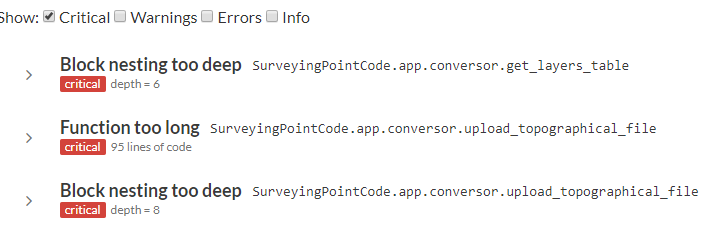
\includegraphics[width=1\textwidth]{CB_2}
	\caption{Puntos críticos del código.}
	\label{fig:CB_2}
\end{figure}

localizados en dos funciones:
\begin{enumerate}

\item \texttt{upload\_topographical\_file()}: En esta función \emph{Codebeat} indica que la profundidad máxima que alcanzan los bucles y condicionales es de 8, y también, que la longitud de la función es de 95 líneas. Como en el resto del código, se podía haber dividido está función en otras más pequeñas, pero en esté caso se ha primado leer una sola ver los datos y crear todos los elementos interpretados en un solo recorrido.

\item \texttt{get\_layer\_table()}: En esta función \emph{Codebeat} indica que la profundidad máxima que alcanzan los bucles y condicionales es de 8. Como en el caso anterior, se podía haber dividido está función en otras más pequeñas, pero en esté caso se ha primado también  leer una sola ver los datos y crear todos los elementos interpretados en un solo recorrido.
\end{enumerate}

Se han realizado cambios en el código para intentar reducir estos puntos críticos, quedando en análisis finalmente:

\begin{figure}[!h]
	\centering
	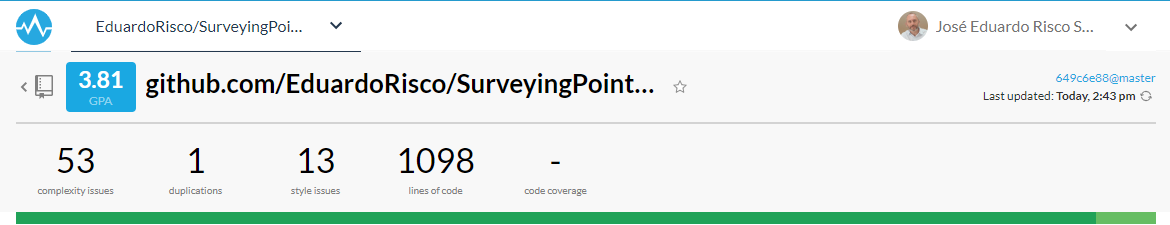
\includegraphics[width=1\textwidth]{CB_3}
	\caption{Resultado del 2º análisis con \emph{Codebeat}.}
	\label{fig:CB_3}
\end{figure}

La puntuación final se ha mejorado poco, 0.01, pero se han logrado evitar dos puntos críticos:

\begin{figure}[!h]
	\centering
	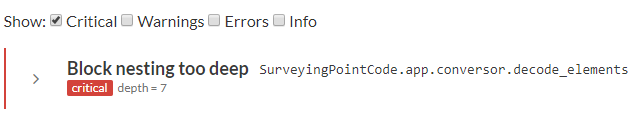
\includegraphics[width=1\textwidth]{CB_4}
	\caption{Reducción de 2 puntos críticos del código.}
	\label{fig:CB_4}
\end{figure}

El resultado del análisis de la calidad del código es muy bueno, se ha puesto mucho interés durante el proyecto en desarrollar un código de calidad que sea fácilmente entendible, extensible y reusable.

Por último, hay que indicar que el informe con la calidad del código se encuentra disponible en el siguiente enlace:\\
 \url{https://codebeat.co/projects/github-com-eduardorisco-surveyingpointcode-master}
 